\chapter{Fundamentals}
This chapter covers the fundamentals necessary to understand the methods presented and their application.
It is divided into a section on neural networks and one on the used software and frameworks.
The former starts with the principle of a neural network.
It continues with an explanation of the network architectures multilayer perceptrons and convolutional neural networks.
The first one serves as an example of how networks work in general.
The second one is more suited for image processing and outperforms the first one in this task.
It continues with an explanation of the required steps to train the network for achieving the wanted use case.
Finally, methods and parameters are examined that improve the overall performance of a neural network.
The latter explains which software and frameworks support building and training a model.

\section{Artificial Neural Networks}
\label{sec:neural-networks}
This section examines the types of neural networks that are important for this work.
Furthermore, it explains how these types are built and trained in order to achieve the wanted use case.
General knowledge is taken from \cite{Goodfellow-et-al-2016} and \cite{cs231n}.

\subsection{Overview}
\label{sec:neural-networks-overview}
Artificial neural networks are vaguely inspired by the biological neural networks that constitute animal brains for recognizing patterns.
Its task is being a universal approximator for any unknown function $f(x) = y$ where $x$ is the input and $y$ the output.
There are two conditions that need to be fulfilled.
One is the relation of $x$ and $y$ and the other is the presence of numerical data.
So every data like images, text or time series must be translated.
The complexity of the approximated function depends on the use case but usually it is highly non-linear.
General use cases for neural networks embrace classification, clustering, and regression.

Classification means the network divides given data like images into categories by recognizing patterns.
This is the task used in this work.
The correct category of each input is given as an additional label.
Therefore, the network learns the correlation between data and labels.
Kind of a downside here is that every input must be labeled by human knowledge beforehand.
This kind of learning is called supervised learning because each predicted category by the network needs to be compared with the ground truth label.
Use cases are for example the classification of cars in images or even the type of car in an image or whether an email is spam.
Again, it all depends on the wanted use case and given data.

Clustering divides data into clusters or groups, respectively, but without requiring labels.
Therefore, this learning type is called unsupervised learning.
So it is kind of a classification task with dynamic category creation.
Use cases are comparing data to each other and finding similarities or anomalies.
Because unlabeled data occurs way more often than labeled data in real world examples, a network can train on a broader range of related data and probably gets more accurate than a classification one.

Regression is the prediction of a future event by establishing correlations between past events and future events.
A simple use case is the prediction of the price of a house given its size and the size-price data pairs of different houses.
A more advanced use case is the prediction of hardware breakdowns by establishing correlations of already known data.
\subsection{Multilayer Perceptron}

\input{tex/fundamentals/neural_networks/mlp/theorie.tex}
\input{tex/fundamentals/neural_networks/mlp/activations.tex}
\input{tex/fundamentals/neural_networks/mlp/hyperparameters.tex}
\subsubsection{Training}
\label{sec:mlp-training}
Thus far optimal weights and biases were assumed.

Expressing the activation of every node with \thmref{eq:perceptron-sum} would get very complex with only a few nodes.
Hence, a matrix notation is the way to go in the long run.
First, for every layer a vector is build
\subsection{Convolutional Neural Networks}
\label{sec:neural-networks-convolutional-neural-networks}
Convolutional neural networks are suited for image processing tasks because they perform better than the multilayer perceptrons architecture regarding the accuracy and the number of parameters \cite{Lecun98} \cite{LeCun1998cnn}.
The reason for the first one is most likely that they are invariant regarding the position of an object within an image.
Convolutional neural networks do not have an as strict separation in multiple layers as multilayer perceptrons do.
They rather have a pool of several layers which can be arbitrarily connected, repeated, and tuned with respect to their parameters to fulfill one's needs as illustrated in \figref{fig:cnn-layers}.
\begin{figure}
	\centering
	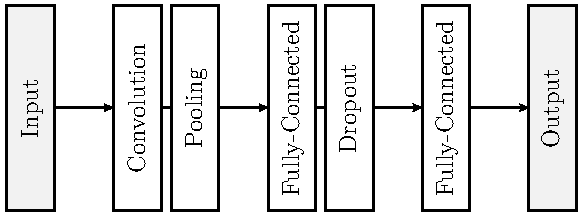
\includegraphics[]{images/cnn_layers.pdf}
	\caption[Layers of a convolutional neural network]{Layers of a convolutional neural network. Each combination of convolutional layer and pooling layer or fully-connected and dropout can be arbitrarily repeated. Moreover, pooling layers and dropout regularization layers are optional.}
	\label{fig:cnn-layers}
\end{figure}
Commonly, convolutional layers are combined with pooling layers and fully-connected layers with dropout regularization layers.
However, the latter combinations are optional.
Each of them is explained in the following sections.
Combinations and repetitions of those layers with their own hyperparameters are called architecture.
Usually, convolutional and pooling layers manipulate the input and the resulting activations before fully-connected layers appear.
There are different proposed architectures with their weights and biases available.
The most common ones are AlexNet \cite{Krizhevsky:2012:ICD:2999134.2999257}, VGG \cite{Simonyan15}, GoogLeNet \cite{szegedy2015} and, ResNet \cite{He2016ResNet}.

\subsubsection{Convolutional Layer}
\label{sec:cnn-convolutional-layer}
The most important layer is the convolutional layer.
As the name suggests it performs a convolution with a filter matrix of arbitrary size on an input matrix of arbitrary size.
Let's say the input matrix is an image $\vec{X} \in \mathbb{R}^{m \times n}$.
The filter matrix $\vec{K} \in \mathbb{R}^{i \times j}$ contains $i \cdot j$ weights of the network.
The filter is now slid across the image and performs a dot product within its window.
\figref{fig:convolution} illustrates the following operation.
In reference to the figure the kernel covers the four elements in the top right corner of the input image.
Hence, the dot product multiplication for this setup yields $5 \cdot 1+4 \cdot -1+1 \cdot -1+3 \cdot 1=3$.
This result is stored in a new matrix at its corresponding place.
At the end, this matrix will hold all values of the convolution operation.
After each calculation of the dot product, the filter matrix moves.
The corresponding step size is called stride.
A stride of 1 moves the filter one pixel or element, respectively.
There can be a different stride along the $x$-axis and $y$-axis.
When the filter has moved across the whole input, the resulting matrix is completely filled up like the one in the figure.
This resulting matrix is called a feature map, because the convolution extracted features from its input.
\begin{figure}
	\centering
	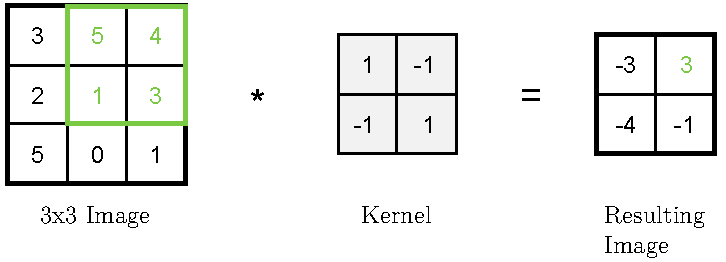
\includegraphics{images/convolution.pdf}
	\caption[Convolution of an Image with a Kernel]{Convolution of an image and a kernel. The $2 \times 2$ kernel is sled across the $3 \times 3$ image and performs a dot product multiplication within its window each time. Here, the kernel moves with a stride of 1, which results in the shown image on the right, the so called feature map.}
	\label{fig:convolution}
\end{figure}
Doing this operation the feature map is always smaller than the input.
Sometimes this is not desirable, because this means a loss in information.
If multiple convolutions are performed, the feature map constantly shrinks until no feature can be extracted anymore or only rough ones.
Thus, a padding $p$ can be applied to the input.
This means surrounding the input with $p$ rounds of zeros like it is illustrated in \figref{fig:convolution-padding} with $p=1$.
The convolution operates like usual, just on a larger input.
\begin{figure}
	\centering
	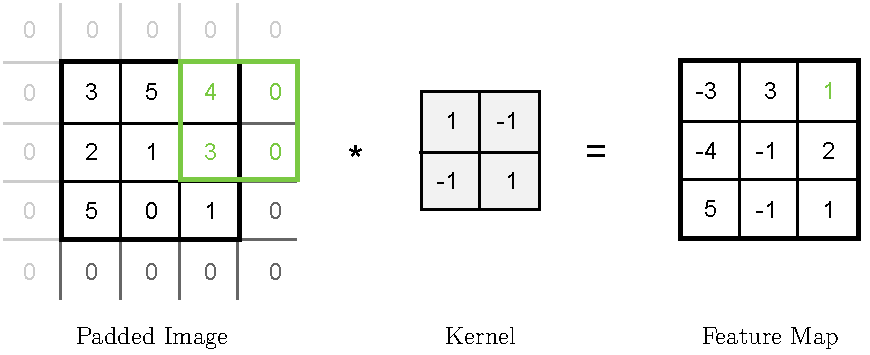
\includegraphics{images/convolution_padding.pdf}
	\caption[Convolution of a Padded Image with a Kernel]{Convolution of a padded image with a $2 \times 2$ kernel. The $3 \times 3$ image is surrounded with zeros for inducing its size to the feature map. However, the convolution operates like usual, just on a larger input. If the amount padding is odd, a padding at the right and at the bottom is preferred.}
	\label{fig:convolution-padding}
\end{figure}
In practical terms, there are two common conventions for convolutions: valid and same.
The former defines that no padding is applied and therefore a kind of valid convolution is performed, because only the real input is minded.
This means that the feature map has a size of $\vec{F} \in \mathbb{R}^{m-i+1 \times n-j+1}$.
The latter means, that the size of the feature map equals the one of the input.
How much padding $p$ needs to be applied can be calculated by comparing each matrix shapes and using
\begin{align}
	m &= m+2p-i+1 \\
	p &= \frac{i-1}{2}
\end{align}
as a general equation.
However, this only covers the padding height.
If the image or filter are not symmetrical, the padding along the width needs to be calculated as well by replacing $m$ with $n$ and $i$ with $j$.
Another remark is, that in computer vision filter sizes usually are odd.
There can be two reasons for this.
First, the filter has a center which helps to tell where exactly the filter points to.
Second, the padding $p$ is even.
Otherwise, it needs to be rounded up for a correct mathematical representation, but only used on two sides of the image like it is shown in the figure with the help of transparency.
Only the padding at the right and at the bottom are taken into account for creating a filter matrix with the same shape of the original input.

The kernel in the figure would find top-left to bottom-right diagonal lines, because those are the pixels weighted most.
Like this but with slightly larger kernels and different weights more complex features can be found.
It is also possible to perform multiple different convolutions on the same input for finding different features.
They are stored as a matrix, where every feature represents the depth of the feature map.
This whole process solves the limitation to a fixed position of features of the multilayer perceptrons architecture.
Even if, for example, a digit covers only have the image, all features are found, because the kernel is moved over the image and not single neurons or filters are responsible for single pixels.
Furthermore, because features are found by a moving filter, convolutional neural networks need way less weights and biases due to the possibility of reusing them.
The accuracy compared to multilayer perceptron networks is improved by concatenating several convolutions.
That means a convolution is performed on the feature map of an earlier convolution.
First, rough features like edges are found, and the deeper it gets into the network, the finer the features get.
\subsubsection{Pooling Layer}
\label{sec:cnn-pooling-layer}
After obtaining features using a convolutional layer a pooling layer can be inserted working on their activations.
Pooling serves as a spatial dimension reduction.
This is done by moving a filter $\vec{K} \in \mathbb{R}^{i \times j}$ with a given stride $s$ over an input $\vec{I} \in \mathbb{R}^{u \times v}$ that compresses the information or values, respectively, within its window.
However, the depth is usually not compressed and stays the same.
The objective of this process is to remove unnecessary information while keeping important features and improving computational power as less spatial information is available.
Hence, fewer weights and biases are needed which in turn improves training time.
\figref{fig:pooling} illustrates the pooling process for a max pooling operation in practical terms.
A max pooling filter $\vec{K}_{\text{max}}$ yields the maximum within its window as the result.
Moving such a $2 \times 2$ filter over an $4 \times 4$ input $\vec{I}$ with a stride of $s=2$ yields a matrix with each maximum at its corresponding position.
The maximum of the red colored $2 \times 2$ window is 7, hence, this number comes up in the result.
The other windows are processed identically.
The size of the result of an arbitrary pooling operation can be calculated with \eqref{eq:feature-map-shape} and $\dim \left( \vec{F} \right)_3 = \dim \left( \vec{I} \right)_3$.
Another pooling type is mean pooling.
Hereby, the result of each window is the mean of all its values.
In many architectures max pooling outperforms mean pooling \cite{Scherer2010}, however, in general, the type of pooling is problem-specific.
As it can be seen, pooling layers do not have learnable parameters only hyperparameters.
\begin{figure}
	\centering
	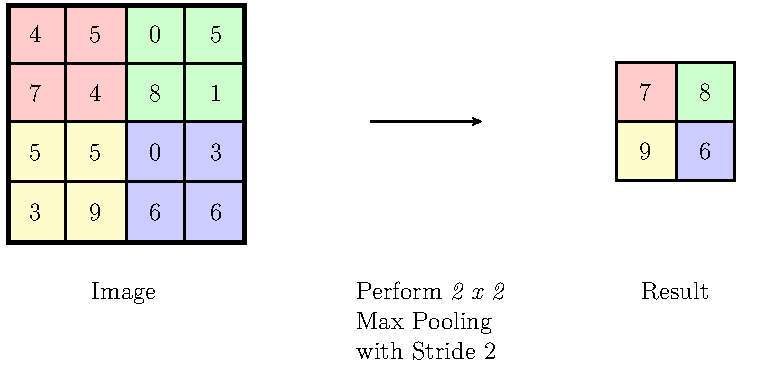
\includegraphics{images/pooling.pdf}
	\caption[Max pooling with $2 \times 2$ filter and stride $2$]{Max pooling with $2 \times 2$ filter $\vec{K}_{\text{max}}$ across a $4 \times 4$ input $\vec{I}$ with a stride of $s=2$. Within each window, the maximum of its values is computed. Finally, this yields a matrix with each maximum at its corresponding position.}
	\label{fig:pooling}
\end{figure}
\subsubsection{Fully-Connected Layer}
\label{sec:cnn-fully-connected}
The last part of a convolutional neural network mostly consists of at least one fully connected layer.
Such a layer is identical to a perceptron layer in \figref{fig:multilayer-perceptron} but uses the outputs or activations, respectively, of the previous convolutional or pooling layer.
The objective is to combine several features that were detected and use them as attributes for classifying the input.
Due to the weights, some attributes are more significant than others.
For example, if four legs and a long snout are found, there is a dog in the image and not a cat.
If the task is to distinguish only between cats and dogs, the snout feature is weighted more than the leg feature.
For preventing overfitting and improving generalization, a fully-connected layer can be combined with the dropout regularization technique \cite{Srivastava:2014:DSW:2627435.2670313}.
This drops out nodes randomly during training with a given probability, i.\,e. changing their incoming and outgoing weights temporarily to zero.
Hence, their weights are not adapted.
The interpretation of the activations of the last fully-connected layer in the architecture is simplified by applying an additional softmax function that squashes them into a range of 0 and 1, whereas the sum of all equals 1, to represent percentages of confidence or a probability distribution, respectively \cite{Bishop2006}.
The prediction $\hat{y}$ of a class $c$ manipulated with the softmax function can be written as
\begin{equation}
	\label{eq:softmax}
	\hat{y}_c = \frac{\exp(a^{[L]}_c)}{\sum_{j}^{n_y} \exp(a^{[L]}_j)}
\end{equation}
where $\vec{a}^{[L]}$ are the activations of the last layer.
Because the softmax manipulation outputs a probability distribution, it can only be performed when the classes are mutually exclusive, i.\,e. when only one class is correct.
Otherwise, for multi-label classification, a sigmoid function can be used, that squashes each output of the network into a range of 0 and 1.
The softmax or sigmoid manipulation corresponds to the output block in \figref{fig:cnn-layers}.
Combining the last fully-connected layer with a dropout layer is not desirable because this would remove some predictions of classes.
\subsection{Train a Neural Network}
\label{sec:neural-networks-training}
So far optimal weights and biases were assumed in all examples, that exactly model a desired function $f(\vec{x, \vec{W}, \vec{B}}) = \vec{y}$ where $\vec{W}$ and $\vec{B}$ store all parameters of a network.
But in practical terms, they need to be found first for generating the desired output.
This starts by collecting or generating and preparing a dataset from which the network can find correlations by changing the weights and biases.
Then, those parameters are randomly initialized.
Furthermore, the data samples of the dataset are used as input and are feed-forwarded through the network yielding a classification $\hat{\vec{y}}$.
This classification is evaluated by a cost function.
That result is back-propagated through the network by computing its gradients for changing the weights and biases.
The forward pass and backward pass are repeated with different samples until an termination condition is satisfied.
\figref{fig:training} illustrates this process.
Each of these steps is covered in the following sections.
\begin{figure}
	\centering
	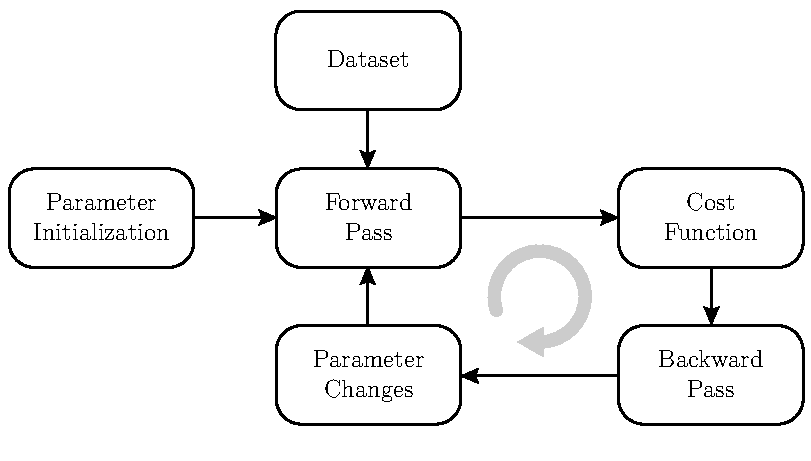
\includegraphics{images/training.pdf}
	\caption[Training process]{Training process. The parameters are initialized once at the beginning. The training process includes the forward pass, the cost function evaluation,the backward pass and the changing of parameters. This is repeated with different data samples.}
	\label{fig:training}
\end{figure}

\subsubsection{Dataset}
\label{sec:dataset-generation}
The whole training process is based on the dataset from which the network is supposed to learn correlations of each input to label.
Usually, a dataset consists of input-label pairs, where the input is the data that is fed into the network and the label is the ground-truth of its class.
In the case of a classification task, the label represents the class.
However, there is no general rule for the amount of data.
It can be said, that more data is better for generalization, but processing too many samples can lead to overfitting the network to the shown data.
The latter means, that the network is trained too long or to intensive on the shown data.
The consequence is, that it adjusts its weights and biases to classify this data perfectly, but cannot reliably generalize to unknown data, because it slightly differs.
Basically, the amount of data depends on the objective of the network.
For classifying whether an image is black or white, only a few training samples would be needed, because this could be classified with the help of few filters, hence, few parameters that need to be adapted.
Is the objective classifying objects within images, it depends on the number of possible objects and their complexity.
If the objects are simple geometric shapes, then not as many samples are needed as if the objects are common objects like type of animals or cars.
There are several datasets available, that are already sorted and labeled, like the MNIST handwritten digits or the ImageNet dataset \cite{Russakovsky:2015:ILS:2846547.2846559}.
Available datasets are not limited to images but may include CAD models like the ModelNet dataset \cite{conf/cvpr/WuSKYZTX15} which is used for the network architecture going to be presented.

Usually, samples of a dataset are split into a training set, test set, and a validation set \cite{James2014}.
The first contains data, the network is trained on.
From this data correlations of each input to label are found.
After an arbitrary number of training steps where parameter changes are executed, the performance of the network is tested on the validation set.
This is data, the network is not trained on.
The objective here is to check if overfitting occurs.
If the loss of the training set decreases, the loss of the validation set has to decrease as well.
This shows that the network still learns and gets better.
If the loss of the training set decreases, but the loss of the validation set stays the same or increases, it is an indicator for overfitting.
This concept is also valid for the accuracy but reversed.
Both cases are visualized in \figref{fig:overfitting}.
The dotted line indicates when training should have been stopped.
\begin{figure}
	\setlength\figureheight{.4\textwidth}
	\setlength\figurewidth{.5\textwidth}
	\centering
	\begin{subfigure}{.5\textwidth}
		\input{images/overfitting_loss.tikz}
		\caption[Loss]{Loss}
	\end{subfigure}%
	\begin{subfigure}{.5\textwidth}
		\input{images/overfitting_accuracy.tikz}
		\caption[Accuracy]{Accuracy}
	\end{subfigure}
	\caption[Indicator of overfitting]{Indicator of overfitting. If loss or accuracy of the validation set do not follow the direction of the one of the training set the network does not generalize. The dashed line represents when training should have been stopped.}
	\label{fig:overfitting}
\end{figure}

The test set is data the network is not trained on as well.
It serves as a final performance check of the network to confirm its general accuracy.
It is bad practice but if no validation set is available, the testing set can be used.
How the dataset is split depends again on the number and complexity of samples and the objective.
However, an equal distribution of samples in terms of samples per class in each set should be minded.
This means, if the network trains mostly on sweatshirts a test set with mostly pants would not yield an acceptable accuracy, because the network does not know these particular features.

For processing the dataset, a one-hot encoding \cite{Harris2012} of the labels can be performed.
Usually, the labels are categorical data.
This means, they contain label or string values, respectively, instead of numeric values, that the networks needs.
For example, there is a fashion variable with the values "boot", "sweatshirt" and "pants".
The network would not know how to interpret these.
Thus, these values need to be converted to numeric values.
Furthermore, if these label values are outputs of the network, it should be easily possible to convert them back from numeric values.
Hence, they are converted to integers that represent a class.
Referring to the example, this results in the numeric values 0, 1 and 2 for the labels "boot", "sweatshirt" and "pants", respectively.
But numeric values have a natural ordered relationship between each other, that neural networks could exploit.
The index of "pants" is higher than the one of "boot", but neither of these classes is better or worse than the other.
Therefore, the indices are one-hot encoded as well.
This means removing the integer representation and inserting binary variables for simulating existing features.
Applying this to the example results in the label vector $\vec{y}^{(2)} = (0, 1, 0)^T$ for the "sweatshirt" label.
This vector has a length of the number of different classes available, where every element is 0 except the one of the corresponding class which is 1.
\tabref{tab:one-hot-encoding} summarizes this approach.
This encoding needs to be performed on each label in the dataset.
\begin{table}[]
	\caption[One-Hot Encoding of Categorical Data]{One-hot encoding of categorical data. First, categorical label values are transformed to numeric values representing a class index. Then, this is replaced with binary variables to represent features, that removes the natural relationship of numeric values to each other. This vector has a length of the number of different classes, where every element is 0 except for the corresponding class which is 1.}
	\label{tab:one-hot-encoding}
	\centering
	\begin{tabular}{l|l|l}
		Categorical   & Integer & One-Hot                   \\ \hline
		"Boot"       & 0       & $\vec{y}^{(1)} = (1, 0, 0)^T$ \\
		"Sweatshirt" & 1       & $\vec{y}^{(2)} = (0, 1, 0)^T$  \\
		"Pants"      & 2       & $\vec{y}^{(3)} = (0, 0, 1)^T$
	\end{tabular}
\end{table}
\subsubsection{Weight Initialization}
\label{sec:training-weight-initialization}
Before the actual training starts, the parameters, the weights and biases, of the network need to be initialized.
If this is done right, i.e. the values are in a range that supports training, optimization will be achieved in lesser or least time.
On the contrary, a converging to optimal values can be impossible.
Reasons for this are the exploding or vanishing of gradients during backpropagation\cite{Hochreiter1991}.
In the backward-pass the gradients are computed for every layer and are passed from end to beginning using the chain rule.
For example, the derivative of the sigmoid function as it can be seen in \figref{fig:sigmoid-derivative} is in the range of $(0, 0.25]$.
If this is multiplied several times, the gradients at the beginning are way smaller than at the end.
If the weights are too small or too large, this effect is intensified.
This is partly true for other activation functions like the ReLU as well.
But here the gradients can become very large too, if the weights are really large.
None of these scenarios is desirable, because the optimal weights are either not reached or skipped.
\begin{figure}
	\setlength\figureheight{.4\textwidth}
	\setlength\figurewidth{.7\textwidth}
	\centering
	\input{images/sigmoid-derivative.tikz}
	\caption{Sigmoid Function and its Derivative}
	\label{fig:sigmoid-derivative}
\end{figure}
This will become more clear in \secref{sec:training-stochastic-gradient} when the expressions of backpropagation are presented.

If the weights are initialized with 0, every neuron would compute the same output.
This leads to an identical gradient for each one and therefore identical parameter updates.
All in all, this would reduce the network to a linear one.
Hence, a common initialization approach is using a Gaussian distribution like $N(\mu, \sigma^2) = N(0, 0.01)$.
However, this way the variance of this distribution of each neuron's output grows with the number of its inputs.
Therefore, a normalization of the variance of each neuron's output to 1 is performed.
This is done by scaling its weights by the square root of its number of inputs.
This can be derived with the $n$ inputs $\vec{x}$ and weights $\vec{w}$ by
\begin{align*}
	Var(z) &= Var \left( \sum_{i}^{n} w_i x_i \right) \\
	&= \sum_{i}^{n} Var \left( w_i x_i \right) \\
	&= \sum_{i}^{n} \left[ E(w_i)^2 \right] Var(x_i) + E \left[ (x_i) \right]^2 Var(w_i) + Var(x_i) Var(w_i) \\
	&= \sum_{i}^{n} Var(x_i) Var(w_i) \\
	&= (n Var(w)) Var(x) \\
\end{align*}
where zero mean inputs and weights are assumed and an identically distribution of all $w_i$ and $x_i$.
Now, $z$ needs to have the same variance as all of its inputs $\vec{x}$, which yields $Var(w) = 1/n$ as every weights variance.
Hence,
\begin{equation}
	\vec{W} = \frac{N(0,1)}{\sqrt{n}}
\end{equation}
initializes the weights.
A similar analysis is done by \cite{Glorot10understandingthe} whose recommendation is
\begin{equation*}
	Var(\vec{w}) = \frac{2}{n_{in} + n_{out}}
\end{equation*}
where $n_{in}$ and $n_{out}$ is the number of neurons in the incoming and outgoing layer, respectively.
Though, this is, for example, not valid for ReLU units, due to their positive mean.
Fortunately, \cite{DBLP:journals/corr/HeZR015} states the initialization
\begin{equation}
	Var(\vec{W})) = N(0,1) * \sqrt{\frac{2}{n}}
\end{equation}
especially for ReLU neurons.

\subsubsection{Feed-Forward Pass}
\label{sec:training-forward-pass}
Let's recall the information, that are needed for the actual training step, i.e. the finding of optimal weights and biases.
Everything starts with a dataset $\mathbb{D}$ containing $m$ pairs of inputs and corresponding labels.
Performing a one-hot encoding on the labels and assuming in general flattened input matrices yields
\begin{equation}
	\label{eq:dataset-one-hot}
	\mathbb{D} =
	\begin{pmatrix}
		\vec{X} & \vec{Y}
	\end{pmatrix}
\end{equation}
where $\vec{X} \in \mathbb{R}^{n_x \times m}$ and $\vec{Y} \in \mathbb{R}^{n_y \times m}$ are representing each input and label as vectors, respectively, forming matrices.
Hereby, $n_x$ represents the size of each input and $n_y$ the number of categories.
Furthermore, there is a neural network with $L$ layers each containing an arbitrarily number of perceptrons.
Expressing the activation of every node with \thmref{eq:perceptron-sum} would get very confusing for a whole network.
Hence, a matrix notation is the way to go in the long run.
First, for every $j$-th node in the $l$-th layer its weights are summarized in a vector
\begin{equation}
	\label{eq:weights-vector}
	\vec{w}^{[l]}_j =
	\begin{pmatrix}
		w^{[l]}_{j,1} & w^{[l]}_{j,2} & \cdots & w^{[l]}_{j,n^{[l-1]}_h}
	\end{pmatrix}^T
\end{equation}
containing single weights, where the superscript in square brackets denotes the layer and the subscript denotes the edge of (target neuron, preceding neuron).
The number of hidden neurons in the $l$-th layer is represented by $n^{[l]}_h$.
These conventions are maintained for all parameters for the rest of this thesis.
The bias of the $j$-th neuron in the $l$-th layer is just a scalar denoted as $b^{[l]}_j$. 
Now, every weight vector and bias can be combined to a matrix and vector, respectively, for each layer.
This yields
\begin{subequations}
\label{eq:parameters}
	\begin{align}
		\vec{W}^{[l]} &=
		\begin{pmatrix}
			\vec{w}^{[l]}_1 & \vec{w}^{[l]}_2 & \cdots & \vec{w}^{[l]}_{n^{[l]}_h}
		\end{pmatrix}^T
		\label{eq:weights}
		\\
		\vec{b}^{[l]} &=
			\begin{pmatrix}
				b^{[l]}_1 & b^{[l]}_2 & \cdots & b^{[l]}_{n^{[l]}_h}
			\end{pmatrix}^T
		\label{eq:biases}
	\end{align}
\end{subequations}
where $\vec{W}^{[l]} \in \mathbb{R}^{n^{[l]}_h \times n^{[l-1]}_h}$ and $\vec{b}^{[l]} \in \mathbb{R}^{n^{[l]}_h}$.

Using these matrices and vectors data can easily be forwarded through the network by building up on \thmref{eq:perceptron-activation}.
The weighted sum of all neurons of the $l$-th layer is computed as
\begin{equation}
	\label{eq:weighted-sum}
	\vec{z}^{[l]} = \vec{W}^{[l]} \vec{a}^{[l-1]} + \vec{b}^{[l]}
\end{equation}
with the activations vector $\vec{a}$.
Putting this in an activation function yields
\begin{equation}
	\label{eq:activations}
	\vec{a}^{[l]} = \phi\left(\vec{z}^{[l]}\right)
\end{equation}
for the $l$-th layers activations.
Performing this for every layer results in 
\begin{equation}
	\label{eq:feedforward}
	\hat{\vec{y}}^{(i)} = f(\vec{x}^{(i)}, \vec{W}, \vec{b})
\end{equation}
as the network's prediction for the $i$-th data sample $\vec{x^}{(i)} \in \mathbb{R}^{n_y}$.
This superscript in round brackets is part of the used convention.

Let's assume that the result is already fed into a sigmoid function and therefore only contains values between 0 and 1.
This prediction needs to be compared with the ground-truth label $\vec{y}^{(i)}$ for checking how good the network performs and, hence, how well the parameters fit.
An example of how these vectors can look like is shown in \tabref{tab:prediction}.
\begin{table}[]
	\centering
	\caption[Example Comparison of One-Hot Encoded Ground Truth Label and Prediction]{Example comparison of an one-hot encoded ground truth label and a softmax prediction. However, the actual ground truth feature has the second smallest probability in the prediction. Therefore, the parameters need to be adjusted.}
	\label{tab:prediction}
	\begin{tabular}{ll}
		Ground-Truth & $\vec{y} = \begin{pmatrix} 0 & 1 & 0 & 0 & 0 \end{pmatrix}^T$                     \\
		Prediction   & $\hat{\vec{y}} = \begin{pmatrix} 0.54 & 0.28 & 0.2 & 0.63 & 0.96 \end{pmatrix}^T$
	\end{tabular}
\end{table}
It can be clearly seen, that the prediction is completely wrong.
The actual ground truth feature has the second smallest probability in the prediction.
In theory, an identical representation would be desirable.
However, in practical terms a slight deviation is normal.
Because finding optimal parameters is a optimization problem, a metric for the performance of the networks is served by a loss function that maps these parameters to a loss value.
The most common loss function for comparing two probability distributions of mutually exclusive classes is the cross entropy loss function.
It is defined as
\begin{equation}
	H(y,p) = -(y \log(p) + (1-y) \log(1-p))
\end{equation}
for a single output representing two classes and as
\begin{equation}
	\label{eq:cross-entropy-loss}
	H(\vec{y}, \vec{p}) = - \sum_{i}^{C} y_i \log (p_i)
\end{equation}
for multiclass classification, where $C$ is the number of classes, $i$ the moving index, $\vec{y}$ the ground truth vector and $\vec{p}$ the predicted probabilities\cite{murphy2013machine}.
Applying the previous notation to this yields
\begin{subequations}
	\begin{align}
		\vec{y} &= \vec{y}^{(i)} \\
		\vec{p} &= \hat{\vec{y}}^{(i)} \\
		C &= n_y
	\end{align}
\end{subequations}
as analogies.
Due to the one-hot encoding of the labels, only the positive class $C_p$ is taken into account in the loss computation.
Hence, \thmref{eq:cross-entropy-loss} is reduced to
\begin{equation}
	\label{eq:cross-entropy-loss-compact}
	H(\vec{y}, \vec{p}) = - y_p \log (p_p)
\end{equation}
where $y_p$ and $p_p$ denote the probability of the positive label and its corresponding prediction, respectively.
A visualization of this expression is shown in \figref{fig:cross-entropy}.
\begin{figure}
	\setlength\figureheight{.5\textwidth}
	\setlength\figurewidth{.8\textwidth}
	\centering
	\input{images/cross-entropy-loss.tikz}
	\caption[Cross-Entropy Loss]{Cross-Entropy Loss. Large deviations in probability are strongly penalized.}
	\label{fig:cross-entropy}
\end{figure}
It can be seen, that large deviations in probability are strongly penalized.
In the range of small deviations the slope of the graph is small which leads to little changes in loss, if the probability difference changes only slightly.
Therefore, both kind of errors are penalized.
Using this loss function for computing a cost that averages all losses yields
\begin{equation}
	\label{eq:cross-entropy-cost}
	J(\vec{x}, \vec{W}, \vec{b}, \vec{y}) = J(\hat{\vec{y}}, \vec{y}) = \frac{1}{m} \sum_{i=1}^{m} H(\vec{y}^{(i)}, \hat{\vec{y}}^{(i)})
\end{equation}
as the cost function.
This function depends on all weights and biases as regression parameters, hence, it is highly dimensional.
Minimizing it with respect to the weights and biases yields optimal parameters.
\subsubsection{Backpropagation with Gradient Descent}
\label{sec:training-gradient-descent}
Due to the non-linearities in the network induced by the activation functions, the minimum of the cost function cannot be computed analytically but numerically.
Using backpropagation \cite{rumelhart1986learning, Goodfellow-et-al-2016} results in a gradient for each parameter.
Depending on these values representing the slope of the parameters, and, hence, their impact on the output, the parameters are changed to move closer to the minimum.
This optimization is done by using the gradient descent algorithm \cite{kiefer1952, robbins1951}.
\figref{fig:gradient-descent} illustrates this approach.
The gradients point into the direction of steepest ascent.
To reach the minimum, those are negated for pointing into the direction of steepest descent.
Finally, the parameters are moved along this direction.
\begin{figure}
	\centering
	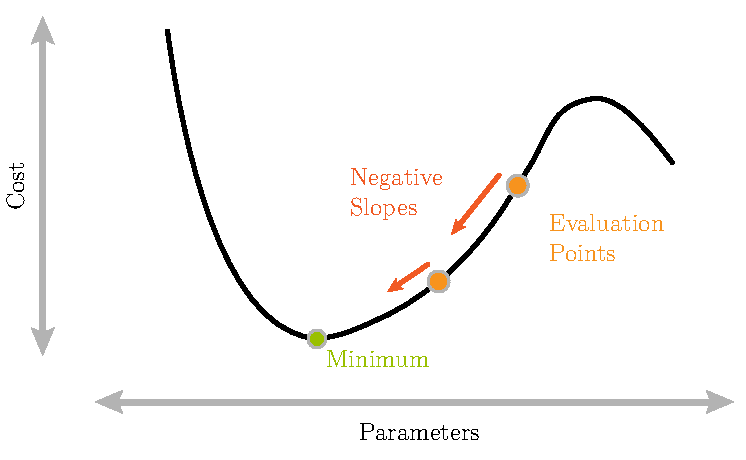
\includegraphics{images/gradient_descent.pdf}
	\caption[Schematic of gradient descent]{Schematic of gradient descent. Cost is evaluated, its negative gradients are computed and the parameters are moved along this direction until the minimum is reached.}
	\label{fig:gradient-descent}
\end{figure}
Following this approach means for the whole network that the cost function is backpropagated layer by layer to the beginning of the network using partial derivatives and the chain rule.
When this is completed, it is known how the parameters are influencing the output and therefore how they need to be changed depending on their slope.

The goal of backpropagation is to compute the partial derivatives
\begin{subequations}
	\label{eq:backpropagation}
	\begin{align}
		\frac{\partial J}{\partial w^{[l]}_{jk}} &= \frac{1}{m_{\text{train}}} \sum_{i}^{m_{\text{train}}} \frac{\partial J^{(i)}}{\partial w^{[l]}_{jk}} \\
		\frac{\partial J}{\partial b^{[l]}_j} &= \frac{1}{m_{\text{train}}} \sum_{i}^{m_{\text{train}}} \frac{\partial J^{(i)}}{\partial b^{[l]}_j}
	\end{align}
\end{subequations}
of the cost function w.r.t. the parameters by averaging the partial derivatives of cost functions of $m_{\text{train}}$ samples from the training set that were passed through the network.
These $m_{\text{train}}$ samples build a so-called batch in this context.
\figref{fig:backpropagation-influences} recaps the data flow in a neuron in the last layer.
By checking stepwise how a parameter directly influences a subsequently one, \eqref{eq:backpropagation} can be written as
\begin{subequations}
	\label{eq:backpropagation-last}
	\begin{align}
		\frac{\partial J}{\partial w^{[L]}_{jk}} &= \frac{\partial z^{[L]}_j}{\partial w^{[L]}_{jk}} \frac{\partial a^{[L]}_{j}}{\partial z^{[L]}_{j}} \frac{\partial J}{\partial a^{[L]}_{j}} \\
		\frac{\partial J}{\partial b^{[L]}_{j}} &= \frac{\partial z^{[L]}_j}{\partial b^{[L]}_{j}} \frac{\partial a^{[L]}_{j}}{\partial z^{[L]}_{j}} \frac{\partial J}{\partial a^{[L]}_{j}}
	\end{align}
\end{subequations}
for the last layer.
How much the activations of the second to last layer influence the cost function is expressed by
\begin{equation}
	\label{eq:backpropagation-activations-last}
	\frac{\partial J}{\partial a^{[L-1]}_{k}} = \sum_{j=1}^{n_y} \frac{\partial z^{[L]}_j}{\partial a^{[L-1]}_{k}} \frac{\partial a^{[L]}_{j}}{\partial z^{[L]}_{j}} \frac{\partial J}{\partial a^{[L]}_{j}}
\end{equation}
where all weighted sums and activations of the output layer are considered.
This needs to be done because layers are fully connected and the activation of one neuron influences every neuron in the next layer.
Especially in the last layer, the activation of one neuron in the second to last layer influences directly the activations of all neurons in the last layer.
Those are directly related to the cost, which is computed by comparing them with the ground-truth values.
Hence, the influences of the activations of the neurons in the second to last layer need to be summed up.
\begin{figure}
	\centering
	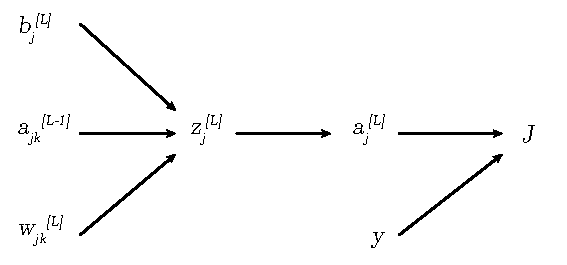
\includegraphics[]{images/backpropagation_influences.pdf}
	\caption[Data flow in a last-layer neuron for backpropagation]{Data flow in a last-layer neuron for backpropagation}
	\label{fig:backpropagation-influences}
\end{figure}
Once \eqref{eq:backpropagation-activations-last} is calculated for the second to last layer, this process can be repeated for all the weights and biases feeding into that layer.
This goes on layer for layer until the first one is reached.
In general,
\begin{equation}
	\label{eq:backpropagation-neuron-error}
	\delta^{[l]}_j = \frac{\partial J}{\partial a^{[l]}_j} \frac{\partial a^{[l]}_{j}}{\partial z^{[l]}_{j}}
\end{equation}
defines the error of the $j$-th neuron in the $l$-th layer.
Combining \eqref{eq:backpropagation-last} and \eqref{eq:backpropagation-neuron-error} yields
\begin{subequations}
	\label{eq:backpropagation-general}
	\begin{align}
		\frac{\partial J}{\partial w^{[l]}_{jk}} &= \frac{\partial z^{[l]}_j}{\partial w^{[l]}_{jk}} \frac{\partial a^{[l]}_{j}} {\partial z^{[l]}_{j}} \frac{\partial J}{\partial a^{[l]}_j} = \frac{\partial z^{[l]}_j}{\partial w^{[l]}_{jk}} \delta^{[l]}_j \\
		\frac{\partial J}{\partial b^{[l]}_{j}} &= \frac{\partial z^{[l]}_j}{\partial b^{[l]}_{j}} \frac{\partial a^{[l]}_{j}} {\partial z^{[l]}_{j}} \frac{\partial J}{\partial a^{[l]}_j} = \frac{\partial z^{[l]}_j}{\partial b^{[l]}_{j}} \delta^{[l]}_j
	\end{align}
\end{subequations}
as the general expressions for backpropagation where
\begin{subequations}
	\begin{align}
		\frac{\partial z^{[l]}_j}{\partial w^{[l]}_{jk}} &= a^{[l-1]}_j \\
		\frac{\partial z^{[l]}_j}{\partial b^{[l]}_j} &= 1 \\
		\frac{\partial a^{[l]}_{j}}{\partial z^{[l]}_{j}} &= \phi'(z^{[l]}_j)
	\end{align}
\end{subequations}
are the derivatives.
Summarizing the gradients of the cost function yields the compact representation
\begin{equation}
	\label{eq:cost-gradient}
	\nabla \vec{J} =
	\begin{pmatrix}
		\frac{\partial J}{\vec{W^{[1]}}} &
		\frac{\partial J}{\vec{b^{[1]}}} &
		\frac{\partial J}{\vec{W^{[2]}}} &
		\frac{\partial J}{\vec{b^{[2]}}} &
		\cdots &
		\frac{\partial J}{\vec{W^{[L]}}} &
		\frac{\partial J}{\vec{b^{[L]}}}
	\end{pmatrix}^T
\end{equation}
containing the influences of all parameters.
Each element points into its direction of steepest ascent with a magnitude.
Hence, each gradient is inverted for pointing into its direction of steepest descent for finding a minimum.
Along each direction, depending on its magnitude each parameter is changed.
This can be expressed by
\begin{subequations}
	\label{eq:learning-rate}
	\begin{align}
		w^{[l]}_{jk}(\tau + 1) &= w^{[l]}_{jk}(\tau) - \gamma \nabla \vec{J}(w^{[l]}_{jk}(\tau)) \\
		b^{[l]}_j(\tau + 1) &= b^{[l]}_j(\tau) - \gamma \nabla \vec{J}(b^{[l]}_j(\tau))
	\end{align}
\end{subequations}
where the hyperparameter $\gamma$ is the learning rate and $\tau$ the iteration step.
This update procedure is done for every batch that is passed through the network.
The updates resulting from a batch are called an iteration.
This is repeated for the whole training set, which is called an epoch.
The objective of the learning rate is to control how much the parameters are adjusted.
The smaller it is, the slower the parameters are moving along the graph to the minimum.
On its way, the slope steadily gets smaller which intensifies this effect.
A similar effect arises by moving over plateaus.
Surely, the minimum will be found more exactly than with a large learning rate, but it would make learning really slow.
However, a large learning rate can steadily overshoot the minimum leading to no convergence.
These effects are roughly exemplified in \figref{fig:learning-rate}.
Thus, a trade-off must be found or an adaption of the learning rate to certain circumstances like the magnitude of the slope is necessary.
\begin{figure}
	\centering
	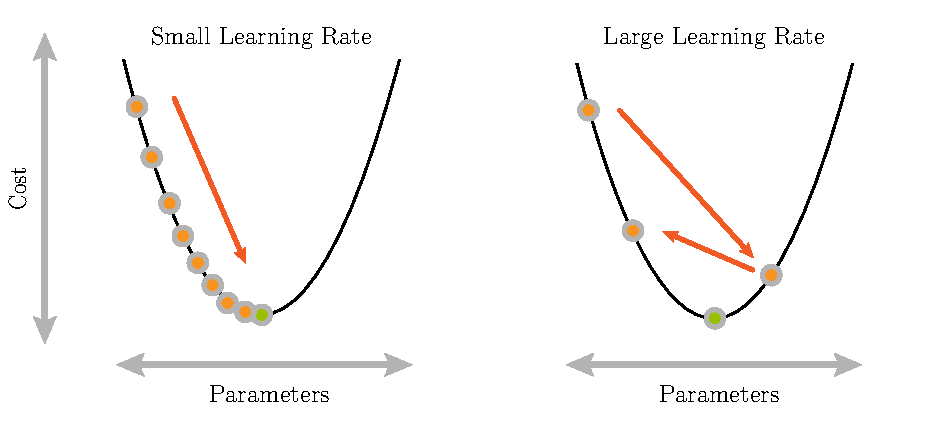
\includegraphics[]{images/gradient_descent_learning_rate.pdf}
	\caption[Comparison of learning rates]{Comparison of learning rates. A small learning rate finds the minimum slowly but more exactly than a high learning rate. However, the latter tends to overshoot the minimum. This is roughly exemplified.}
	\label{fig:learning-rate}
\end{figure}
According to \textit{Bengio} \cite{DBLP:journals/corr/abs-1206-5533} a traditional default value for the learning rate is $\gamma_0 = 0.1$ or $\gamma_0 = 0.01$ for standard multilayer neural networks.
However, it remains a hyperparameter that is problem-specific, hence, only guidelines can be provided.
One of them is, that the learning rate should be greater than $10^{-6}$ and less than $1.0$.
Another approach is decaying the initial learning rate either linearly or exponentially until iteration $\tau$ and then leaving it constant \cite{Goodfellow-et-al-2016}.
The underlying idea is to move quickly to close proximity to the minimum and then carefully to it.
Another common approach is an exponential decay like
\begin{equation}
	\gamma(\tau) = \gamma_0 \exp(-\lambda\tau)
\end{equation}
where $\gamma_0$ is the initial learning rate, $\lambda$ a factor and $\tau$ the iteration step.
The concept of changing the learning rate over time is called learning rate schedule. Its values are arbitrary and do not inevitably need to be results of a decay but can be fixed values that are active depending on the time step $\tau$, for example.

Due to the number of parameters and the use of hidden layers, cost functions are highly dimensional and neither convex nor concave.
An explanation for the latter is, that several combinations of parameters can result in the same loss value.
Hence, there are several local minima in the cost function.
According to \textit{Choromanska et al.} \cite{DBLP:journals/corr/ChoromanskaHMAL14} almost all local minima have very similar function values to the global minimum.
Hence, finding a local one is sufficient.
Having neither a convex nor concave cost function, the function probably has saddle points.
These points are no optimum but have a gradient of $\nabla \vec{J} = \vec{0}$.
The types of critical points are shown in \figref{fig:critical-points}.
\begin{figure}
	\centering
	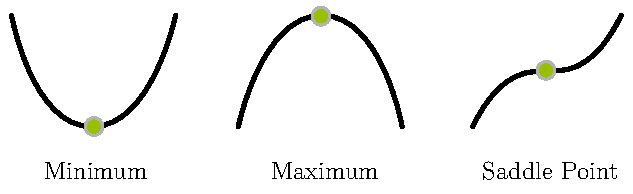
\includegraphics[]{images/gradient_descent_types.pdf}
	\caption{Types of critical points}
	\label{fig:critical-points}
\end{figure}
With this gradient the algorithm would get stuck.
Hence, adding some noise to \eqref{eq:learning-rate} yields
\begin{subequations}
	\begin{align}
		w^{[l]}_{jk} &:= w^{[l]}_{jk} - \gamma \nabla \vec{J}(w^{[l]}_{jk}) + \vec{\varepsilon}(w^{[l]}_{jk}) \\
		b^{[l]}_j &:= b^{[l]}_j - \gamma \nabla \vec{J}(b^{[l]}_j) + \vec{\varepsilon}(b^{[l]}_j)
	\end{align}
\end{subequations}
where $\vec{\varepsilon}$ is a noise vector with mean 0.
Because saddle points are very unstable, adding some noise helps to overcome them.
\subsubsection{Adam Optimization Algorithm}
\label{sec:training-adam}
\subsection{Improving Performance}
\label{sec:neural-networks-improving-performance}
Earlier sections make general recommendations on hyperparameters.
Nevertheless, there is room for improvement.
Finding well-suited hyperparameters is a trial-and-error method and requires much time.
However, there are methods that aim to find a good starting point.
Those are going to be presented in the following.

\subsubsection{Optimal Learning Rate}
\label{sec:improving-performance-learning-rate}
The learning rate is the most important hyperparameter in a neural network.
If it is too small, learning converges exactly, though, really slow.
If it is too large, the minimum is steadily overshot and learning maybe diverges.

\textit{Smith} introduces the cyclical learning rate \cite{DBLP:journals/corr/Smith15a}.
For being cyclical, the learning rate needs a lower and upper bound.
This builds a range of optimal learning rates.
With these values inbetween, the evaluations of the cost function are effectively decreased over time.
Hence, for finding that optimal range, the learning rate is initialized with a very small value and slightly increased after each training step.
For each of the steps the cost function is evaluated.
\figref{fig:optimal-learning-rate-range} shows a typical plot of the cost function against the learning rate on a logarithmic $x$-scale.
\begin{figure}
	\setlength\figureheight{.45\textwidth}
	\setlength\figurewidth{.9\textwidth}
	\centering
	\input{images/optimal_learning_rate_loss.tikz}
	\caption[Optimal Range of Learning Rates]{Optimal Range of Learning Rates Highlighted in Blue. The learning rate is increased exponentially.}
	\label{fig:optimal-learning-rate-range}
\end{figure}
It can be seen, that if the learning rate is small, the cost function does not improve noticeably.
When the learning rate gets into its optimal range, the cost function suddenly becomes smaller.
This continues with a large gradient, until the learning rate exits its optimal range.
This passage is detected when the cost function starts to oscillate.
If the learning rate still gets increased, the cost function starts to diverge eventually.
\textit{Smith} suggests a triangular learning rate policy which first increases the learning rate from the lower bound to the upper bound and then decreases it back to the lower bound.
Each change happens linearly.
The actual learning rate depends on the time step.

Another approach is doing warm restarts of the learning rate after several iterations, hence, it is called Stochastic Gradient Descent with Warm Restarts\cite{DBLP:journals/corr/LoshchilovH16a}.
This is especially combined with the gradient descent algorithm.
The idea behind it is to swing out of a tight local minimum if the algorithm seems to get stuck there.
If well-suited parameters are found for a cost function, the latter can slightly change if the dataset changes.
Hence, the once well-suited parameters lead to a worse cost now.
Therefore, a minimum in a flatter region needs to be found where a slight change has no big impact, i.e. a solution that is more generalized across datasets.
\figref{fig:sgdr-cost} illustrates this scenario.
\begin{figure}
	\centering
	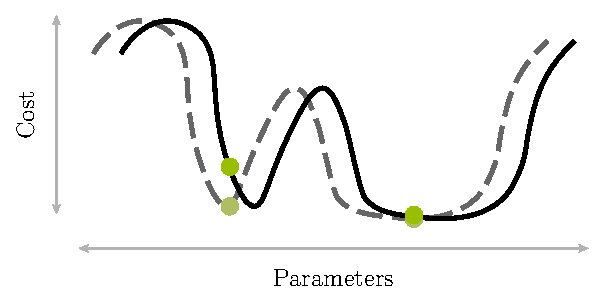
\includegraphics[]{images/sgdr-cost.pdf}
	\caption[Cost Function of Different Datasets]{Cost Function of Different Datasets. If the parameters represent a minimum of a dataset's cost function, the same parameters do not inevitably represent the minimum of a different dataset's cost function.}
	\label{fig:sgdr-cost}
\end{figure}
This algorithm uses a cosine annealing of the learning rate.
This means the learning rate is decreased in the form of half a cosine curve.
This is called a cycle.
After this, it is set to its initial value and the annealing is repeated.
This process is visualized in \figref{fig:sgdr-annealing-normal}.
\begin{figure}
	\setlength\figureheight{.3\textwidth}
	\setlength\figurewidth{.45\textwidth}
	\centering
	\begin{subfigure}{.49\textwidth}
		\centering
		\input{images/sgdr-annealing.tikz}
		\caption{Cosine Annealing}
		\label{fig:sgdr-annealing-normal}
	\end{subfigure}%
	\setlength\figurewidth{.45\textwidth}
	\begin{subfigure}{.49\textwidth}
		\centering
		\input{images/sgdr-annealing-extended.tikz}
		\caption{Extended Cosine Annealing}
		\label{fig:sgdr-annealing-extended}
	\end{subfigure}
	\caption{Annealing of Stochastic Gradient Descent with Warm Restarts}
	\label{fig:sgdr-annealing}
\end{figure}
So, first, the cost in decreased until the learning rate reset happens.
Then, it is possible to overshoot the local minimum that much, that a different one is targeted.
However, this minimum is flat enough that another learning rate restart does not change the targeted minimum.
Due to the objective of finding flat regions it is advisable to steadily extend each learning rate cycle like it is shown in \figref{fig:sgdr-annealing-extended}.
It is assumed, that the more iterations are done, the flatter the found region gets.
Thus, the longer its minimum is searched.
\subsubsection{Optimal Batch Size and Number of Epochs}
\label{sec:improving-performance-batch-size}
The batch size defines how many samples are propagated through the network at once.
Moreover, the adaption of parameters due to backpropagation depends only on the current batch.
This means, $m_{\text{train}}$ in the cost function in \eqref{eq:cross-entropy-cost} and in the partial derivatives in \eqref{eq:backpropagation} can be replaced with a given batch size as long as it is smaller than the actual number of samples in the corresponding set.
For each sample within a batch the gradients of the cost function with respect to all parameters are calculated and finally averaged over all batch samples for yielding how the parameters need to be changed.
That process is repeated for different batches until the whole dataset is propagated forward and backwards.
Then it can be repeated with a shuffled dataset, hence, different batches.

For finding the optimal batch size, the most obvious choices are examined first.
On the one hand, the whole training set can form a batch.
This way the best direction to a minimum can be calculated.
In terms of number of iterations, this method is the best.
However, it is very expensive in terms of resources, because usually the amount of data can not be held in the RAM or GPU.
This means, either more memory needs to be bought or a continual reload of data happens, which slows down the overall training process.
An even more significant downside is that large batch sizes in relation to the dataset result in a worse performance of the model in terms of generalization \cite{DBLP:journals/corr/KeskarMNST16}.
Because the parameter updates follow the best direction to a minimum does not mean, that this minimum is well-suited for other data.
Usually, the model converges to a tight minimum, similar to \figref{fig:sgdr-cost}, due to their frequency.
On the other hand, a batch size of one is used, which is called stochastic.
The parameter updates are noisy and can point into a completely wrong direction, while still pointing along the steepest descent.
Hence, they wander around the cost function and eventually reach the minimum after a long training time.
However, the computing cost of the gradients of a single sample is quite trivial.
Thus, a trade-off must be found for a so-called mini-batch.
One requirement is that the training converges in a reasonable amount of time.
This includes averaging out the noise of the gradients for more accurate steps leading to an earlier convergence.
Hence, the batch size to choose also depends on the learning rate.
A smaller batch size is better suited for a small learning rate due to the noise.
A good balance is found if the batch is small enough to avoid the poor minima but stays in the flatter, better-performing ones.
Another requirement is the computational cost.
Fortunately, vector computing is optimized almost perfectly in most frameworks, resulting in only marginally higher computation cost for a few samples compared to a single one.
Hence, a batch size should be larger than one, usually, and less than the whole training set but the optimal size is only found by trial and error.
Common batch sizes are 32, 64, 128 and 256.

When using mini-batches the number of epochs is a hyperparameter, that can be tuned, as well.
Important is the generalization of the network, while preventing underfitting or overfitting.
Thus, the number of epochs cannot be determined beforehand but depends on the data.
However, the training set needs to be shuffled every epoch, so that different batches are created compared to earlier epochs.
This improves generalization due to the computation of different batch gradients.
\subsubsection{Activation Functions}
\label{sec:improving-performance-activation-functions}
The activation functions of a neural network affect its performance and convergence as well.
Common activation functions are shown in \figref{fig:activation-functions}.
The most common ones are going to be examined.
The sigmoid function recently has fallen out of favor.
One disadvantage is its saturation which leads to a very small gradient.
If this small gradient is often multiplied because of several layers, the gradient gets very small.
This vanishing gradient leads to very small parameter updates.
Furthermore, a well-suited weight initialization is required.
If they are too large, related neurons become saturated and the network will barely learn.
Hence, in both cases, convergence takes a very long time.
Another disadvantage is, that outputs are not zero-centered.
That means, that, for example, if all data is positive, all related gradients point into the same, either positive or negative, direction.
This leads to an undesired zigzag pattern of the parameter updates for several samples.
However, the use of mini-batches smooths out this effect.
The tanh activation function has a zero-centered output, though, the saturation of the output remains.
The ReLU activation function accelerates the convergence process of stochastic gradient descent compared to sigmoid and tanh.
According to \textit{Krizhevsky et al.}, it is six times faster on the CIFAR10 dataset \cite{Krizhevsky2009LearningML} compared to tanh activation functions \cite{Krizhevsky:2012:ICD:2999134.2999257}.
This is due to its linear, non-saturation form.
Another advantage is its simple and light computation.
Furthermore, it makes the activations sparse from the perspective of a neural network.
This means not all neurons are active due to the ReLU being zero for input values below zero.
Hence, the overall network is lighter.
However, its property of the evaluation to zero is also a disadvantage.
This results in a gradient of zero as well and therefore in no related parameter updates.
If the weights are initialized badly or an unfavorable update is applied, for example, due to a too large learning rate, a ReLU unit can die, because its evaluation and the gradient are zero for all further computations.
In this case, a unit is very unlikely to recover.
A solution forms the leaky ReLU, which adds a slight slope of like $\lambda = 0.01$ to the horizontal line of 0, preventing the gradient to become zero.
Hence, the unit can recover.
However, the results of this approach are very inconsistent.

Taking all that information into account yields the recommendation of the ReLU activation function, if the weights and learning rate are chosen carefully
Additionally, the fraction of dead units should be monitored.
If the number is still concerning, leaky ReLU activations should be applied.
The tanh activation should be generally preferred over the sigmoid one.

\begin{figure}
	\setlength\figureheight{.3\textwidth}
	\setlength\figurewidth{.5\textwidth}
	\centering
	\begin{subfigure}{.5\textwidth}
		\centering
		\input{images/threshold-activation.tikz}
		\begin{equation*}
		\phi(x) =
		\begin{cases}
		1 & x \geq \text{Bias $b$} \\
		0 & x < \text{Bias $b$}
		\end{cases}
		\end{equation*}
		\caption{Threshold}
		\label{fig:threshold-activation}
	\end{subfigure}%
	\hfill
	\begin{subfigure}{.5\textwidth}
		\centering
		\input{images/heaviside-activation.tikz}
		\begin{equation*}
		\phi(x) =
		\begin{cases}
		1 & x \geq 0 \\
		0 & x < 0
		\end{cases}
		\end{equation*}
		\caption{Heaviside}
		\label{fig:heaviside-activation}
	\end{subfigure}
	
	\begin{subfigure}{.5\textwidth}
		\centering
		\input{images/relu-activation.tikz}
		\begin{equation*}
		\phi(x) =
		\begin{cases}
		x & x \geq 0 \\
		0 & x < 0
		\end{cases}
		\end{equation*}
		\caption{Rectified Linear Unit}
		\label{fig:relu-activation}
	\end{subfigure}%
	\hfill
	\begin{subfigure}{.5\textwidth}
		\centering
		\input{images/leakyrelu-activation.tikz}
		\begin{equation*}
		\phi(x) =
		\begin{cases}
		x & x \geq 0 \\
		x\cdot \text{Slope $\lambda$} & x < 0
		\end{cases}
		\end{equation*}
		\caption{Leaky Rectified Linear Unit}
		\label{fig:leakyrelu-activation}
	\end{subfigure}
	
	\begin{subfigure}{.5\textwidth}
		\centering
		\input{images/sigmoid-activation.tikz}
		\begin{equation*}
		\phi(x) = \frac{1}{1+\exp(-x)}
		\end{equation*}
		\caption{Sigmoid}
		\label{fig:sigmoid-activation}
	\end{subfigure}
	\caption[Common activation functions]{Plots and equations of common used activation functions. Where the Bias $b$ is the threshold value and $\lambda$ adds a small slope. Usually, the latter is very small like $\lambda=0.01$.}
	\label{fig:activation-functions}
\end{figure}
\subsection{Metrics for Performance Evaluation}
\label{sec:neural-networks-metrics}
There are several common metrics available that, for example, measure the classification accuracy or its precision.
However, they depend on some definitions that will be introduced first.
The positive class of a data sample represents its ground-truth class, while the negative one represents any of the remaining ones, i.\,e. not the positive class.
A true positive $TP$ is a correct prediction of a sample, so the positive class is predicted correctly.
A true negative $TN$ is a correct rejection of a sample, i.\,e. the network classifies this sample correctly as not the positive class.
Furthermore, a false positive $FP$ is a wrong prediction of a sample as the positive class.
The last definition is a false negative $FN$.
This means the network incorrectly predicts a sample as a negative class.
Their connection is visualized in \figref{fig:confusion-matrix} showing the so-called confusion matrix \cite{Fawcett:2006:IRA:1159473.1159475} for the example class Class A.
This needs to be repeated for each class in a dataset.
\begin{figure}
	\centering
	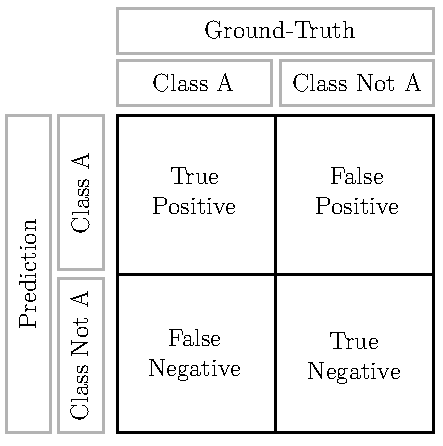
\includegraphics[]{images/confusion_matrix.pdf}
	\caption[Confusion matrix]{Confusion matrix for class A.}
	\label{fig:confusion-matrix}
\end{figure}
One metric is the accuracy
\begin{equation}
	ACC = \frac{TP + TN}{TP + TN + FP + FN}
\end{equation}
of a class.
Averaging all class accuracies yields the network accuracy.
This states how many samples the network correctly classifies.
However, this metric's results are not reliable for the real performance, because it highly depends on the dataset and its balance, among others.
If it is unbalanced there are, for example, more samples in a well-classifiable class than in a bad one, hence, the accuracy is shifted.
The precision or positive predicted value of a class measures how accurate the related predictions are and is calculated by
\begin{equation}
	\label{eq:metric-precision}
	PPV = \frac{TP}{TP + FP}
\end{equation}
where the denominator refers to the total positive results.
Furthermore, the recall or true positive rate metric measures how good all positives of a class are found by
\begin{equation}
	\label{eq:metric-recall}
	TPR = \frac{TP}{TP + FN}
\end{equation}
where the denominator refers to the actual positives of a class.
Both \eqref{eq:metric-precision} and \eqref{eq:metric-recall} must be calculated for each class to get a complete overview of the dataset.
A simplified representation of the confusion matrix can be prepared by entering only the number of predictions per class.
This is beneficial for a quick overview of the prediction distribution of multi-class classifications.
Similar to \figref{fig:confusion-matrix} each row represents a predicted class, while the columns represent the ground-truth classes.
Each prediction of the samples of a ground-truth class are summed per class and entered at the corresponding cell.
\section{Software}
This section focuses on explaining which software and frameworks are used for implementing the network and generating the dataset in this work.

\subsection{Tensorflow}
\label{sec:software-tensorflow}
Tensorflow is a free framework in particular for machine learning tasks.
It was originally developed by Google Brain for internal Google use and got finally licensed for open source. 
Mathematical operations are designed as a symbolic graph.
After its creation, any operation inside can be executed and only needs the computation of its dependent operations.
Every computation involves tensors.
A tensor is a generalization of scalars, vectors, and matrices independent on their dimension.
Hence, a definition of every tensor's size is important for a cost-effective creation and computation of the graph.
Due to the symbolic graph, it is possible to define a neural net with an input and output layer and steadily feed and compare different tensor values.
\subsection{Blender}
\label{sec:software-blender}
Blender \cite{blender} is a free and open source 3D creation suite to model, texture and animate objects.
Furthermore, it supports importing existing models and manipulating them.
Additionally, an API interface is provided, that can be used with the programming language Python, to control every function of Blender.
This eases repetitive tasks tremendously.

%Every object in Blender has its own coordinate system.
%Hence, a way of expressing points of one coordinate system in another would be useful.
%It is necessary to define a world coordinate system $\mathcal{W}$ with the origin $\vec{o}_\mathcal{W} = (0,0,0)^T$ and the rotation $\vec{r}_{\mathcal{W}} = (0,0,0)^T$, where each element of the latter represents a rotation around the $x$-, $y$- or $z$-axis, respectively, in radians.
%This system contains every other system.
%Now another coordinate system $\mathcal{L}$ is created, of course, inside the world coordinate system.
%However, $\mathcal{L}$ can be translated and rotated in comparison to $\mathcal{W}$.
%Hence, every coordinate system has a rotation matrix $\vec{R}$ in Euler representation and a translation vector $\vec{t}$ that stores how they are rotated and translated to every other coordinate system.
%Considering $\mathcal{L}$ and $\mathcal{W}$ yields
%\begin{align}
%	\vec{R}_{\mathcal{L} \rightarrow \mathcal{W}} &= \vec{R}_{\mathcal{W} \rightarrow \mathcal{L}}^{-1} \\
%	\vec{t}_{\mathcal{L} \rightarrow \mathcal{W}} &= - \vec{t}_{\mathcal{W} \rightarrow \mathcal{L}}
%\end{align}
%as properties, where the subscript indicates the transfer.
%Transferring the coordinates of an arbitrary local point $\vec{x}_{\mathcal{L}}$ into corresponding coordinates $\vec{x}_{\mathcal{W}}$ of the reference coordinate system is done by using
%\begin{equation}
%	\vec{x}_{\mathcal{W}} = \vec{R}_{\mathcal{L} \rightarrow \mathcal{W}} \cdot \vec{x}_{\mathcal{L}} + \vec{t}_{\mathcal{L} \rightarrow \mathcal{W}}
%\end{equation}
%as the general expression.